\section{Introduction}
\label{sec:intro}

The subject of this report is to present an overview of the state of the art in (large scale) computer vision and image processing (CV\&IP). 
Since this is a very large research area, the focus of this report is mostly on three main research questions in CV\&IP:
\begin{enumerate}
\item {\bf Visual salience:} How can the CV system determine automatically the most visual salient region(s) in an image?\label{item:sal}
\item {\bf Object/scene identification:} How can the CV system automatically determine weather two images, potentially taken with different cameras under different viewing conditions and transformations, represent the same object/scene?\label{item:ident}
\item {\bf Object detection and scene understanding:} How can the computer recognise automatically to what visual category the object/scene captured in an image belongs to? \label{item:und}
\end{enumerate}

Few of the numerous applications related to the visual saliency (\ref{item:sal}) are:
\begin{itemize}
\item Automatic target detection (see fig. \ref{fig:sal})
\item Robot navigation using salient objects
\item Image and video compression
\item Automatic cropping/centering images for display on small portable screens
\item Tumor detection in mammograms, etc.
\end{itemize}

\begin{figure}[H]
\begin{center}
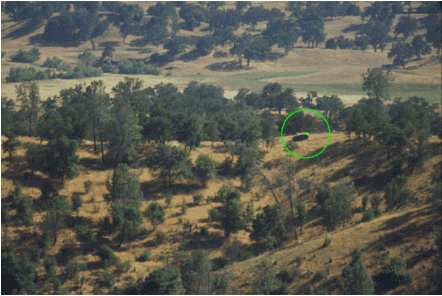
\includegraphics[width=0.8\textwidth]{fig/saliency}
\end{center}
\caption{Example of a saliency model detecting the vehicle as being the most salient object ina complex scene.}
\label{fig:sal}
\end{figure}

Few of the numerous applications related to object/scence identification (\ref{item:ident}) are:
\begin{itemize}
\item Stereo and wide-baseline matching
\item Image panorama stiching/creation
\item Automatic reconstruction of 3D scenes
\item Individual wildlife photo-identification (see figs.  \ref{fig:photoid} and \ref{fig:woodphotoid}), etc.
\end{itemize}

\begin{figure}[H]
\begin{center}
\includegraphics[width=0.8\textwidth]{fig/photoid}
\end{center}
\caption{Example species with sufficient spot pattering what could be useful for automated photo-identification: (a) whale shark (with reference area),
(b) spotted  tree frog, (c) northern quoll, (d) Amazon spotted frog, (e) striped blue crow and (f) mangrove snake.}
\label{fig:photoid}
\end{figure}

\begin{figure}[H]
\begin{center}
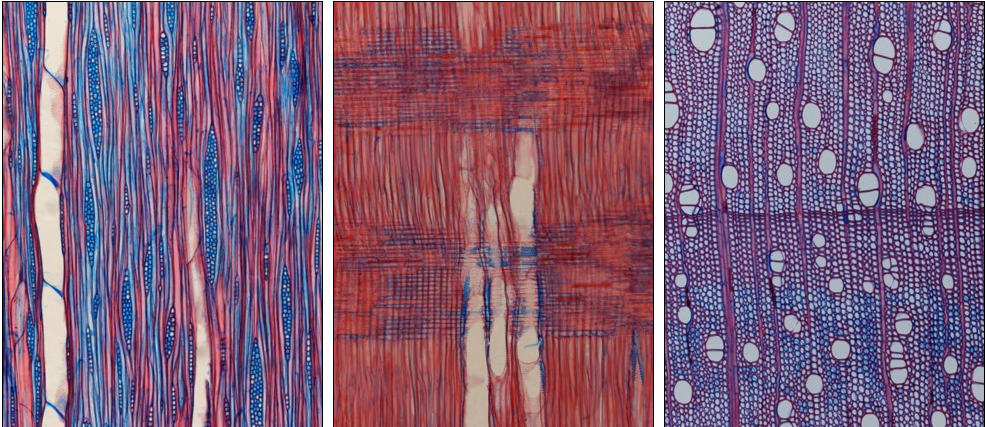
\includegraphics[width=0.8\textwidth]{fig/woodphotoid}
\end{center}
\caption{Left to right: tangential, radial and cross (transversal) sections of stained wood Acer.}
\label{fig:woodphotoid}
\end{figure}

Automatically understading the semantics of an object/scene (\ref{item:und}) have numeral applications like:
\begin{itemize}
\item Image search engines
\item Organizing photo collections
\item Autonomous driving
\item Human machine interaction, etc.
\end{itemize}

This is the most complex and high-level computer vison task, with the goal of making machines see like humans and be able to infer both general principles as well as current situaitons from images. Example of a trained system for scee categorization is shown on fig.\ref{fig:mitdemo}.
\begin{figure}[H]
\begin{center}
\includegraphics[width=0.8\textwidth]{fig/mitdemo}
\end{center}
\caption{MIT Scene Recognition Demo. \url{http://places.csail.mit.edu/demo.html}}
\label{fig:mitdemo}
\end{figure}

The overview is by no means complete, it rather tries to summarise the research in the field along the above three questions in the last years. 
These questions have been chosen having in mind the problems defined in other sciences whcih can be helped by computer science, more precisely by the developments in CV\&IP.

The report is structured along the three main products of CV\&IP reserach, namely, scientific publications in section \ref{sec:pubs}, software in section \ref{sec:soft} and datasets in section \ref{sec:db}. Each section gives examples of the work related to each of the three research questions. Some potential scientific aplications are shown in section \ref{sec:app}.

The goal of this report is not only to summarize, but is also an attempt to identify suitable "niche" for scientifical domain-driven (applied) research in CV\&IP at NLeSc. The conclusions and recommendations are given is section \ref{sec:conc}.